\documentclass[journal,12pt,twocolumn]{IEEEtran}
\usepackage[utf8]{inputenc}
\usepackage{amsmath}
\usepackage{amssymb}
\usepackage{listings}
\usepackage{physics}
\newcommand{\myvec}[1]{\ensuremath{\begin{pmatrix}#1\end{pmatrix}}}
\let\vec\mathbf
\usepackage{graphicx}
\graphicspath{ {./images/} }

\title{Assignment 3
\\Linear Programming }
\author{Swati Mohanty (EE20RESCH11007) }
\date{October 2020}

\begin{document}

\maketitle


\section{Problem}
Minimise and Maximise $Z=x+2y$ subject to $x+2y\geq100$; $2x-y\leq0$; $2x+y\leq200$; $x,y\leq0$.
\section{Solution}
In order to obtain the maximum and minimum value we need to solve the system of inequalities. By plotting the graph of the equations, the common area is obtained. The corners that define the region are A(0,50) ; B(20,40) ; C(50,100)  and D(0,200).
\\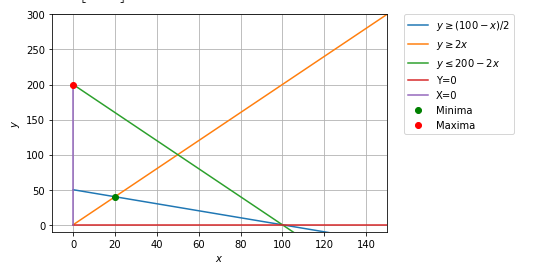
\includegraphics[width=10cm, height=5cm]{plot.jpg}
\\Solving for Z a these points we get
\begin{align}
    Z = x + 2y
    \\
    Maximum Z = 400 ; Minimum Z = 100
\end{align}
The above set of linear programming can be solved by using PulP in python which is a Linear Programming modeler. This optimization module returns the same values of maximum and minimum as obtained from the classical computation.
The following python code generates the equation of circle
\\Link : https://github.com/Swati-Mohanty/EE5600/tree/master/Assignment%203
\end{document}